\subsection{Sistemas de extracci\'on}

\noindent
\justify

Los m\'etodos industrializados m\'as utilizados en el sector alimenticio emplean extracci\'on \textit{s\'olido - l\'iquido} y con \textit{fluido supercr\'itico (SFE)}$^{\cite{Liadakis2003}}$. 

\subsubsection{Sistemas convencionales $\rightarrow$ \textit{Extracci\'on s\'olido - l\'iquido}}

\noindent
\justify

El dis\~no y selecci\'on del sistema de extracci\'on depende, en gran medida, del compuesto objetivo y de las propiedades f\'isicas tanto del material a extraer como del producto. 

\begin{table}[h!]
\begin{adjustbox}{max width = \textwidth}
\begin{tabular}{|p{2.5cm}|p{2cm}|p{10cm}|}
\hline
\textbf{Modalidad} & \textbf{Tipo} & \textbf{Descripci\'on} \\ \hline
\multirow{3}{*}{\begin{tabular}[c]{@{}l@{}}\textbf{Modo de} \\ \textbf{operaci\'on}\end{tabular}} & Extracci\'on por lotes & La extracci\'on se desarrolla en contenedores llenos con el material s\'olido a extraer. Es ineficiente debido a las paradas de planta por \textit{carga} y \textit{descarga} de material. \\ \cline{2-3}
 & Extracci\'on \textit{semi} continua & Con la idea de incrementar la eficiencia de extracci\'on, se desarrolla una operaci\'on de extracci\'on en serie con m\'ultiples recipientes conectados a la misma l\'inea de solvente, el cual se satura de extracto al pasar por cada uno de ellos. \\ \cline{2-3}
  & Extracci\'on continua & El material a extraer es cargado y descargado de manera continua. Se emplean diferentes sistemas de transporte, tanto para los procesos de filtrado como de inmersi\'on en solvente. No es recomendable para extracciones que requieran presiones distintas a la atmosf\'erica. \\ \hline
\multirow{2}{*}{\begin{tabular}[c]{@{}l@{}}\textbf{Principio de} \\ \textbf{trabajo}\end{tabular}} & Extracci\'on de etapa simple & Emplea un recipiente de una etapa para la extracci\'on por inmersi\'on. La inmersi\'on debe presentar agitaci\'on para tener un m\'argen m\'inimo de eficiencia de extracci\'on. \\ \cline{2-3}
 & Extracci\'on \textit{multi} etapa & Utiliza un sistema de operaci\'on contracorriente (propio de sistemas \textit{semi} continuos). El solvente entra en contacto, primero, con la matriz s\'olida de menor concentraci\'on de extracto hacia el de mayor concentraci\'on.  \\ \hline
\end{tabular}
\end{adjustbox}
\caption{Clasificaci\'on de sistemas de extracci\'on convencionales.}
\label{compara}
\end{table}

\noindent
\justify

Los solventes m\'as empleados consisten en agua, hidrocarburos (como el hexano), alcoholes y las mezclas entre ellos a diferentes proporciones.

\newpage

\noindent
\justify

La tendencia sobre el dise\~no de extractores se enfoca en el mejoramiento de la eficiencia y desempe\~no de extracci\'on. Implica el compromiso entre la \textit{simplicidad} del n\'umero de partes m\'oviles y los sistemas de transporte, bombas y bandas transportadoras, y la \textit{eficiencia} del proceso de eluci\'on del solvente. 

\paragraph{Rotocel}

\noindent
\justify

El extractor \textit{Rotocel} es un sistema de extracci\'on por percolaci\'on desarrollado por Blonox en 1960. Se trata de un tanque giratorio con 18 compartimientos de fondo poroso. El material es rociado en cada celda con diferentes concentraciones de solvente recirculado tipo \textit{contracorriente} (como se obersva en la Figura \ref{rotocel}): el solvente rociado en la primera celda corresponde a solvente con cierto grado de saturaci\'on de extracto (proviene de material procesado de otros compartimientos), mientras que el material de la \'ultima celda se roc\'ia con solvente puro.

\begin{figure}[h!]
	\centering
	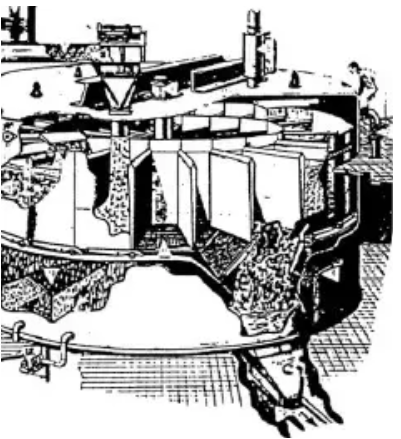
\includegraphics[width=0.5\textwidth]{Images/rotocel.PNG}
	\caption{Extractor Rotocel.}
	\label{rotocel}
\end{figure}

\noindent
\justify

Una rotaci\'on del sistema dura m\'as de una hora, dependiendo de la solubilidad extractiva, y requiere de una energ\'ia rotacional m\'inima debido a que la fuerza de fricci\'on ejercida por el material en cada celda no es de una magnitud considerable. Se conoce como sistema extractor de ``cama profunda", porque cuenta con una profundidad de 1.8 a 3 metros. 

\newpage

\paragraph{Carrousel}

\noindent
\justify

En 1990, el extractor \textit{Carrousel} fue desarrollado mediante la fusi\'on de las licencias Krupp y Extraktionstechnik. Este tipo de extractor puede tener di\'ametros de hasta $15.3 [m]$.

\begin{figure}[h!]
	\centering
	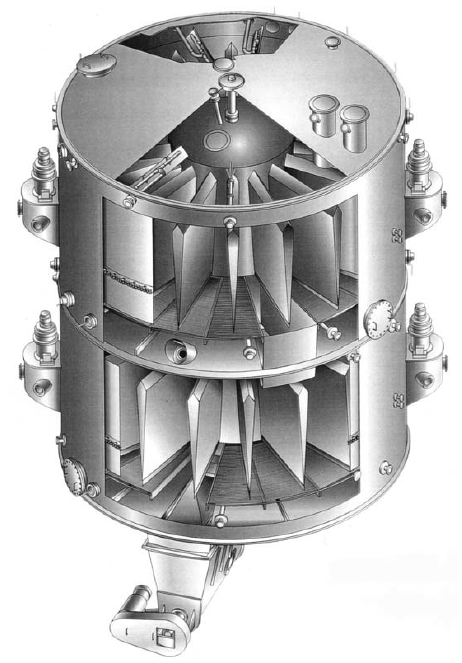
\includegraphics[width=0.4\textwidth]{Images/carrousel.PNG}
	\caption{Interior de un extractor tipo carrousel de doble piso$^{\cite{Liadakis2003}}$.}
	\label{carrousel}
\end{figure}

\noindent
\justify

Presenta el mismo principio de funcionamiento que el sistema de extracci\'on tipo Rotocel, con la diferencia de que el marco de los compartimientos de extracci\'on gira sobre una bandeja de tamiz est\'atica; estructura apreciada en la Figura \ref{tamiz}. 

\begin{figure}[h!]
	\centering
	\begin{subfigure}[b]{0.48\textwidth}
		\centering
		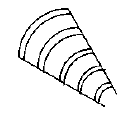
\includegraphics[width=0.5\textwidth]{Images/Original.PNG}
	\caption{Segmento original conc\'entrico.}
	\end{subfigure}
	\hfill
	\begin{subfigure}[b]{0.5\textwidth}
		\centering
		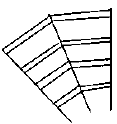
\includegraphics[width=0.48\textwidth]{Images/Actual.PNG}
	\caption{Segmento actual.}
	\end{subfigure}
	\caption{Segmento del fondo de la bandeja de tamiz de un extractor Carrousel$^{\cite{Liadakis2003}}$.}
	\label{tamiz}
\end{figure}

\noindent
\justify

De esta manera, se mejora la transferencia de masa debido a que las part\'iculas se mantinen en constante movimiento.

\paragraph{Pretratamiento}

\noindent
\justify

La eficiencia de extracci\'on est\'a directamente relacionada con la preparaci\'on del material s\'olido a extraer. Peque\~nos tama\~nos de part\'icula son ventajosos debido a la baja resistencia a la difusi\'on entre part\'iculas. Sin embargo, conseguir tama\~nos de part\'icula cercanos al polvo $\left( < 200 \left[ \mu m \right] \right)$ involucra grandes esfuerzos en procesos de trituraci\'on y molienda. Es com\'un emplear como \textbf{pretratamiento mec\'anico} sistemas de molienda de operaci\'on continua; entre ellos: \textit{molinos de rodillos} y \textit{molinos de martillos}, como se aprecia en la Figura \ref{pret}.

\begin{figure}[h!]
	\centering
	\begin{subfigure}[b]{0.5\textwidth}
		\centering
		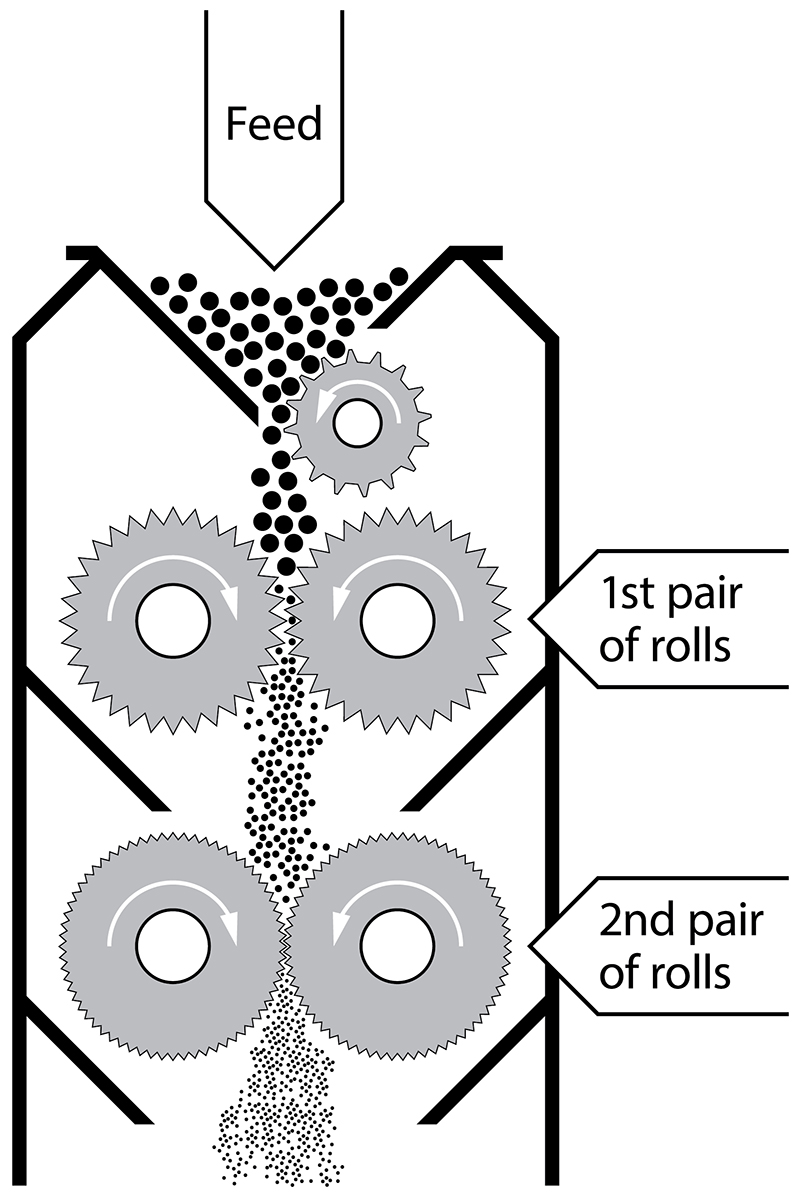
\includegraphics[width=0.7\textwidth]{Images/Rodilloss.png}
	\caption{Molino de rodillos.}
	\end{subfigure}
	\hfill
	\begin{subfigure}[b]{0.5\textwidth}
		\centering
		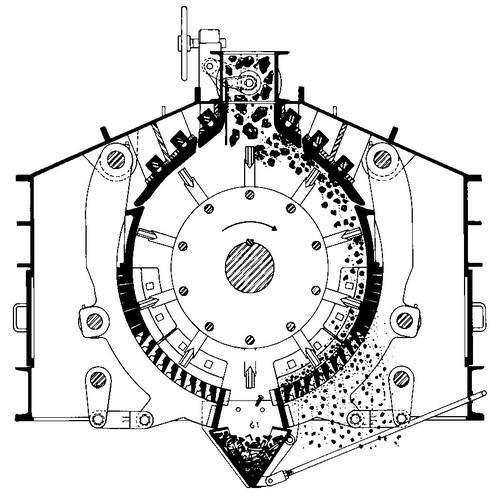
\includegraphics[width=0.9\textwidth]{Images/Martillos.jpg}
	\caption{Molino de martillos.}
	\end{subfigure}
	\caption{Sistemas de pretratamiento mec\'anico.}
	\label{pret}
\end{figure}

\noindent
\justify

En la industria alimenticia es com\'un realizar un \textbf{pretratmiento t\'ermico} para incrementar la eficiencia extractiva durante la producci\'on de aceites con altos valores proteicos, entre ellos: semillas de algod\'on, soja, semillas de s\'esamo y man\'i. Este tratamiento consiste mantener el material solido cerca del $10 \%$ de humedad a temperaturas de $90 - 95 \degree C$.

\paragraph{Recuperaci\'on del solvente}

\noindent
\justify

Una vez obtenida la mezcla solvente - extracto es necesario separarlos a trav\'es de procesos de destilaci\'on. Una vez obtenido el extracto, se pueden realizar procesos de extracci\'on posteriores para limpiarlo de compuestos indeseados, enriquecerlo de otros compuestos o para desarrollar una modificaci\'on qu\'imica.

\subsubsection{Extracci\'on con Fluido Supercr\'itico (SFE)}

\noindent
\justify

La extracci\'on mediante fluido supercr\'itico, especialmente la extracci\'on con dioxido de carbono $\left(CO_2 \right)$, est\'a establecida a una escala industrial y presenta una amplia gama de aplicaciones, entre ellas: producci\'on de caf\'e descafeinado; extracto de l\'upulo; y producci\'on de ingredientes naturales provenientes de hierbas, ra\'ices y aceites esenciales.

\noindent
\justify

El sistema de extracci\'on con fluido supercr\'itico se puede apreciar en la Figura \ref{co2} y consiste de un sistema de presurizaci\'on, un recipente a presi\'on donde ocurre la extracci\'on, otro donde se realiza la separaci\'on y recuperaci\'on del solvente y un par de intercambiadores de calor.

\begin{figure}[h!]
	\centering
	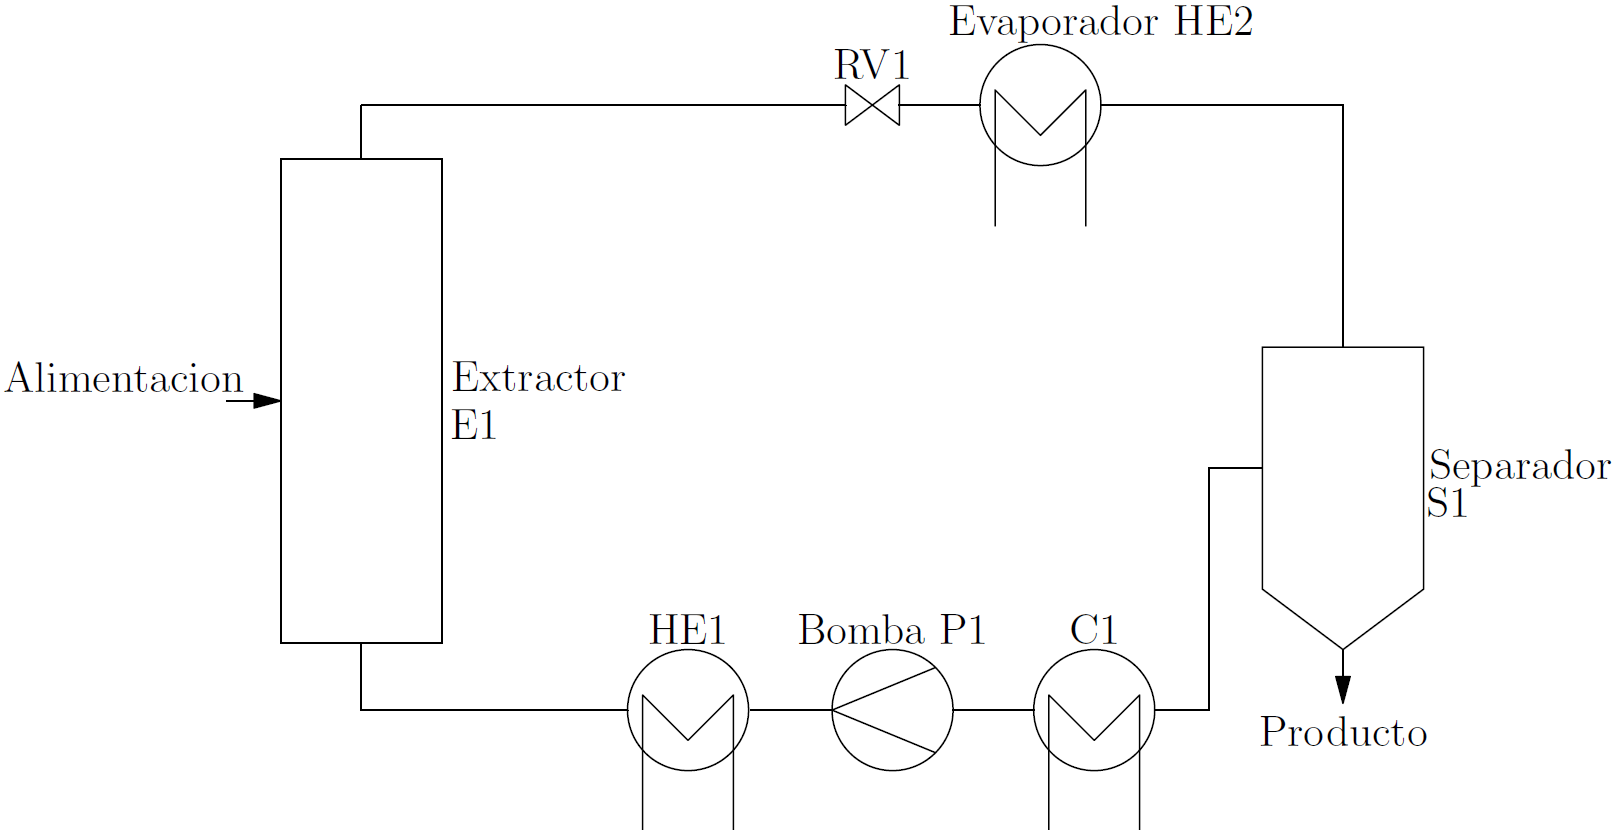
\includegraphics[width=\textwidth]{Images/SFE-CO2/Equipos.PNG}
	\caption{Flujo de trabajo de la extracci\'on con $CO_2$ supercr\'itico.}
	\label{co2}
\end{figure}

\noindent
\justify

El diagrama termodin\'amico del proceso se puede apreciar en la Figura \ref{termo}, del cual se pueden desarrollar balances energ\'eticos.

\begin{figure}[h!]
	\centering
	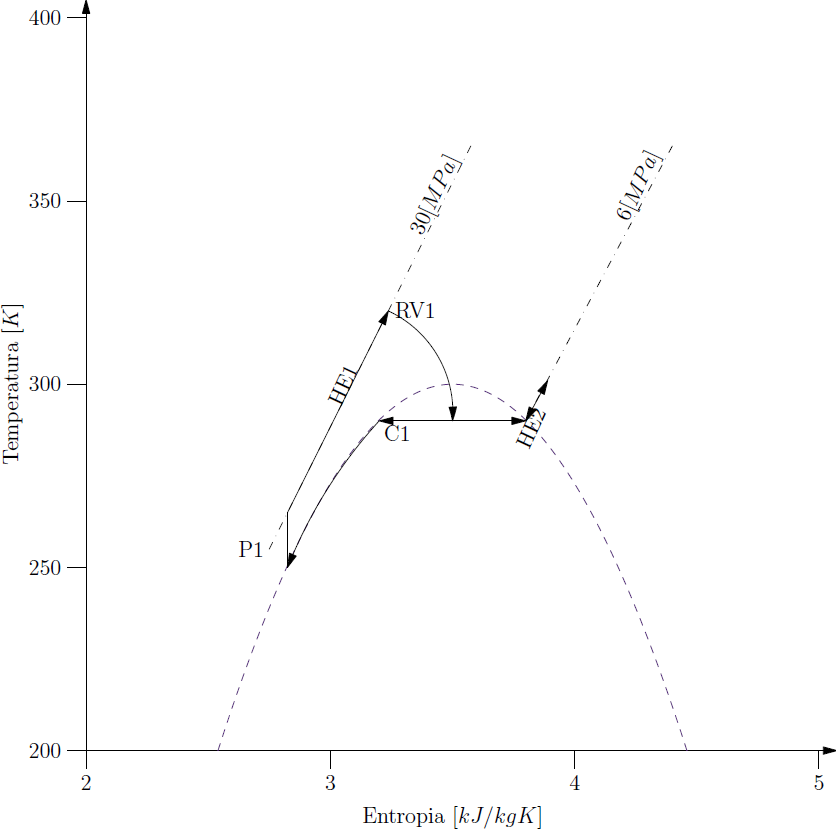
\includegraphics[width=\textwidth]{Images/SFE-CO2/TermoCO2.PNG}
	\caption{Diagrama termodin\'amico T-S.}
	\label{termo}
\end{figure}

\noindent
\justify

Despu\'es de entrar a la zona de l\'iquido saturado en el chiller \textit{C1}, el fluido es lugo comprimido por la bomba \textit{P1}. El incremento de presi\'on se produce de manera casi reversible (isentr\'opicamente). El calentador \textit{HE1} incrementa la temperatura del fluido hasta la temperatura de extracci\'on. Debido a la expansi\'on adiab\'atica que ocurre en la v\'alvula \textit{RV1}, por el efecto Joule-Thompson, el di\'oxido de carbono se enfr\'ia hasta llegar a las condiciones de saturaci\'on. Para facilitar la separaci\'on entre el extracto y el solvente $\left(CO_2 \right)$, el fluido se evapora completamente justo antes de entrar al separador \textit{S1} al pasar por el evaporador \textit{HE2}.

